% HL：直角三角形 斜边+一直角边 全等
\documentclass[tikz,border=4pt]{standalone}
\usepackage{ctex}
\usepackage{amsmath}
\usetikzlibrary{decorations.markings}
\begin{document}
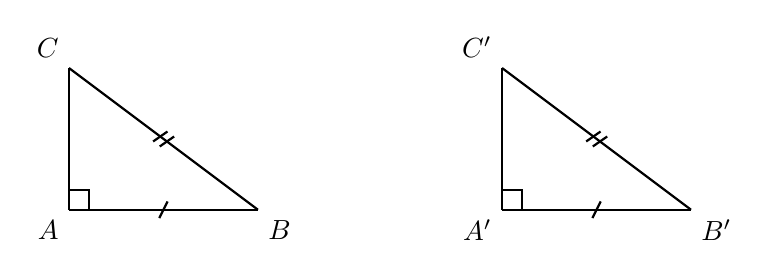
\begin{tikzpicture}[scale=1.0, thick,
  tick/.style={postaction={decorate, decoration={markings,
    mark=at position 0.5 with {\draw (-1.5pt,-3pt) -- (1.5pt,3pt);}}}},
  ticktwo/.style={postaction={decorate, decoration={markings,
    mark=at position 0.5 with {\draw (-2.5pt,-3pt) -- (-0.5pt,3pt);
                               \draw (0.5pt,-3pt)  -- (2.5pt,3pt);}}}}]
  % 左三角形
  \begin{scope}
    \coordinate (A) at (0,0);
    \coordinate (B) at (2.4,0);
    \coordinate (C) at (0,1.8);
    \draw[tick]    (A) -- (B);
    \draw[ticktwo] (B) -- (C);
    \draw          (A) -- (C);
    \draw (0.25,0) -- (0.25,0.25) -- (0,0.25);
    \node[below left]  at (A) {$A$};
    \node[below right] at (B) {$B$};
    \node[above left]  at (C) {$C$};
  \end{scope}
  % 右三角形（全等）
  \begin{scope}[xshift=5.5cm]
    \coordinate (A) at (0,0);
    \coordinate (B) at (2.4,0);
    \coordinate (C) at (0,1.8);
    \draw[tick]    (A) -- (B);
    \draw[ticktwo] (B) -- (C);
    \draw          (A) -- (C);
    \draw (0.25,0) -- (0.25,0.25) -- (0,0.25);
    \node[below left]  at (A) {$A'$};
    \node[below right] at (B) {$B'$};
    \node[above left]  at (C) {$C'$};
  \end{scope}
\end{tikzpicture}
\end{document}
